\section{Методика использования разработанного программного средства}
\label{sec:manual}

В данном разделе будут описаны изменения в методике использования разработанного программного средства по сравнению
с методикой использования, описанной в дипломном проекте~\cite{my_diploma}.

Таким образом, данный раздел не может считаться полноценным руководством пользователя и должен
использоваться в сочетании с соответствующим разделом дипломного проекта.
Несмотря на это, для удобства раздел включает в себя все базовые понятия, необходимые для использования программного средства,
и может считаться краткой справкой по разработанному программному средству.

\subsection{Системные требования}
\label{sec:manual:requirements}

Для запуска разработанного ПС требуются следующие компоненты:
\begin{itemize}
  \item операционная система на базе GNU/Linux;
  \item установленный интерпретатор языка программирования Ruby версии 2.2 или выше;
  \item установленная библиотека SDL версии 2.0.5;
  \item установленная библиотека librsvg версии 2.40.16;
  \item установленная библиотека sdl2\_ttf версии 2.0.14;
  \item установленная библиотека librsvg версии 2.40.16.
\end{itemize}

\subsection{Входные данные симуляции}
\label{sec:manual:input}

Входными данными для симуляции являются файл сценария симуляции и файл схемы сооружения.

\subsubsection{Файл сценария симуляции}
\label{sec:manual:input:scenario}

Файл сценария симуляции использует предметно"=ориентированный язык.
Пример сценария симуляции был представлен на рисунке~\ref{sec:development:preprocessor:scenario_dsl_listing}.
% Пример сценария симуляции представлен на рисунке~\ref{sec:manual:scenario_dsl_listing}.
%
% \begin{figure}[ht!]
%   \centering
%   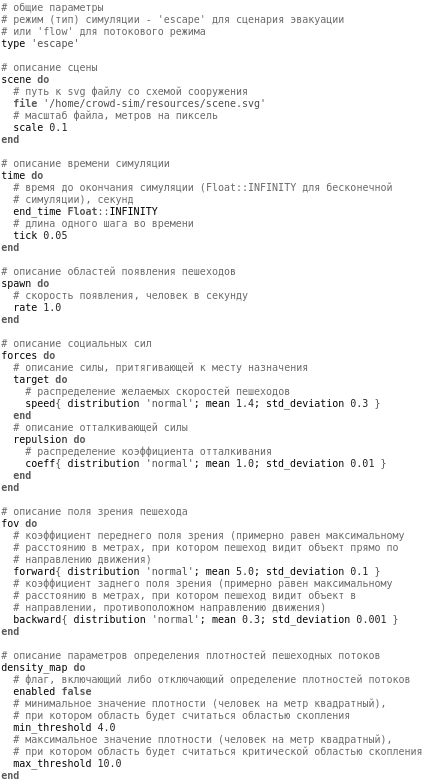
\includegraphics[width=\dimexpr\linewidth-4.5em\relax]{masters_sim_params_example}
%   \caption{Пример сценария симуляции}
%   \label{sec:manual:scenario_dsl_listing}
% \end{figure}

Описание всех полей представлено в примере сценария симуляции. Подробнее остановимся только на поле type.

Поле type задает режим симуляции и может иметь два значения.

Первое значение "--- ''flow'' "--- означает работу в режиме потока.
Блоки, помеченные как области появления людей, будут генерировать новых пешеходов в соответствии со скоростью появления,
заданной в секции spawn полем rate.
В этом режиме условием окончания симуляции является достижение времени, указанного в поле end\_time секции time.
Основное предназначение режима "--- поиск слабых мест в помещениях, где часто скапливаются пешеходы.
Чаще всего используется в сочетании с функцией по поиску мест скопления людей.
При достижении условия окончания симуляции все модули завершают свою работу без каких-либо дополнительных сообщений.

Второе значение "--- ''escape'' "--- означает работу в режиме эвакуации.
Блоки, помеченные как области появления людей, сгенерируют единственного пешехода (вне зависимости от настройки rate в секции spawn).
Условием окончания симуляции является достижение всеми пешеходами своей конечной цели.
Основным предназначением режима является определение характеристик времени эвакуации из определенного сооружения.
При достижении условия окончания симуляции модуль отображения результата выводит текстовое сообщение с
характеристиками времени эвакуации. Характеристики включают в себя минимальное и максимальное время эвакуации,
среднее время эвакуации, а также дисперсию и стандартное отклонение времен эвакуации.
Для выхода из данного состояния необходимо нажать клавишу <<пробел>>.


\subsubsection{Файл схемы сооружения}
\label{sec:manual:input:building_scheme}

Файл схемы сооружения основан на формате векторной графики SVG.
В реализованном ПС поддерживаются три элемента SVG "--- line, rect и circle.

Пример схемы сооружения представлен на рисунке~\ref{sec:manual:input:building_scheme:svg_listing}.

\begin{figure}[!ht]
  \centering
  \begin{subfigure}[!htb]{0.45\textwidth}
    \centering
    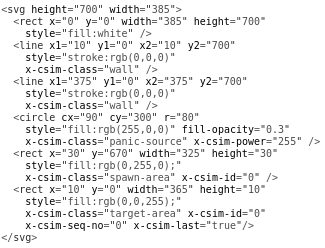
\includegraphics[scale=1.0]{masters_scene_example_text}
    \caption{}
  \end{subfigure}
  \begin{subfigure}[!htb]{0.45\textwidth}
    \centering
    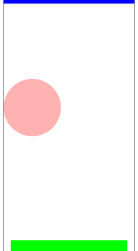
\includegraphics[scale=2.0]{masters_scene_example_pic}
    \caption{}
  \end{subfigure}
  \caption{Пример простой схемы сооружения: а "--- текстовый листинг схемы;
           б "--- схема в виде картинки}
  \label{sec:manual:input:building_scheme:svg_listing}
\end{figure}

В файле допускается использование любых элементов SVG, однако для симуляции будут иметь значение только те элементы, которым проставлен атрибут x-csim-class.
Атрибут x-csim-class отвечает за тип данного элемента.  Возможные значения данного атрибута:
  wall (препятствие),
  spawn"=area (место появления людей),
  target"=area (место назначения людей "--- промежуточное или конечное),
  panic"=source (источник паники).

Описания элементов wall, spawn"=area и target"=area было дано в дипломном проекте, остановимся на элементе panic"=source.
Для элементов с классом panic"=source должен быть проставлен атрибут x-csim-power.
Он задает силу данного источника паники, и должен иметь значение от 0 до 255
(0 "--- источник не распространяет панику, 255 "--- источник распространяет максимальный уровень паники).
Элементы класса panic"=source должны быть элементами circle, при этом желательно делать их прозрачными
(чтобы было возможность наблюдать за пешеходами и другими элементами).

\subsubsection{Запуск программного средства}
\label{sec:manual:launch}

Для запуска в режиме реального времени нужно выполнить следующую команду:
cat \$PATH\_TO\_SCENARIO \-|\- preprocessor/run.rb \-|\- \\ core/target/release/core \-|\- animator/animator animator/resources/person\_1.svg 1.0,
где \$PATH\_TO\_SCENARIO "--- путь к файлу со сценарием симуляции.
